\documentclass[en]{university}

\course{Artificial Intelligence}
\subject{}
\professor{}

\begin{document}

\setupdocument

\section{}
\subsection{}
Bayesian network for each step of the problem is shown in figure \ref{fig:bayes-net}.
\begin{figure}[htbp]
    \centering
    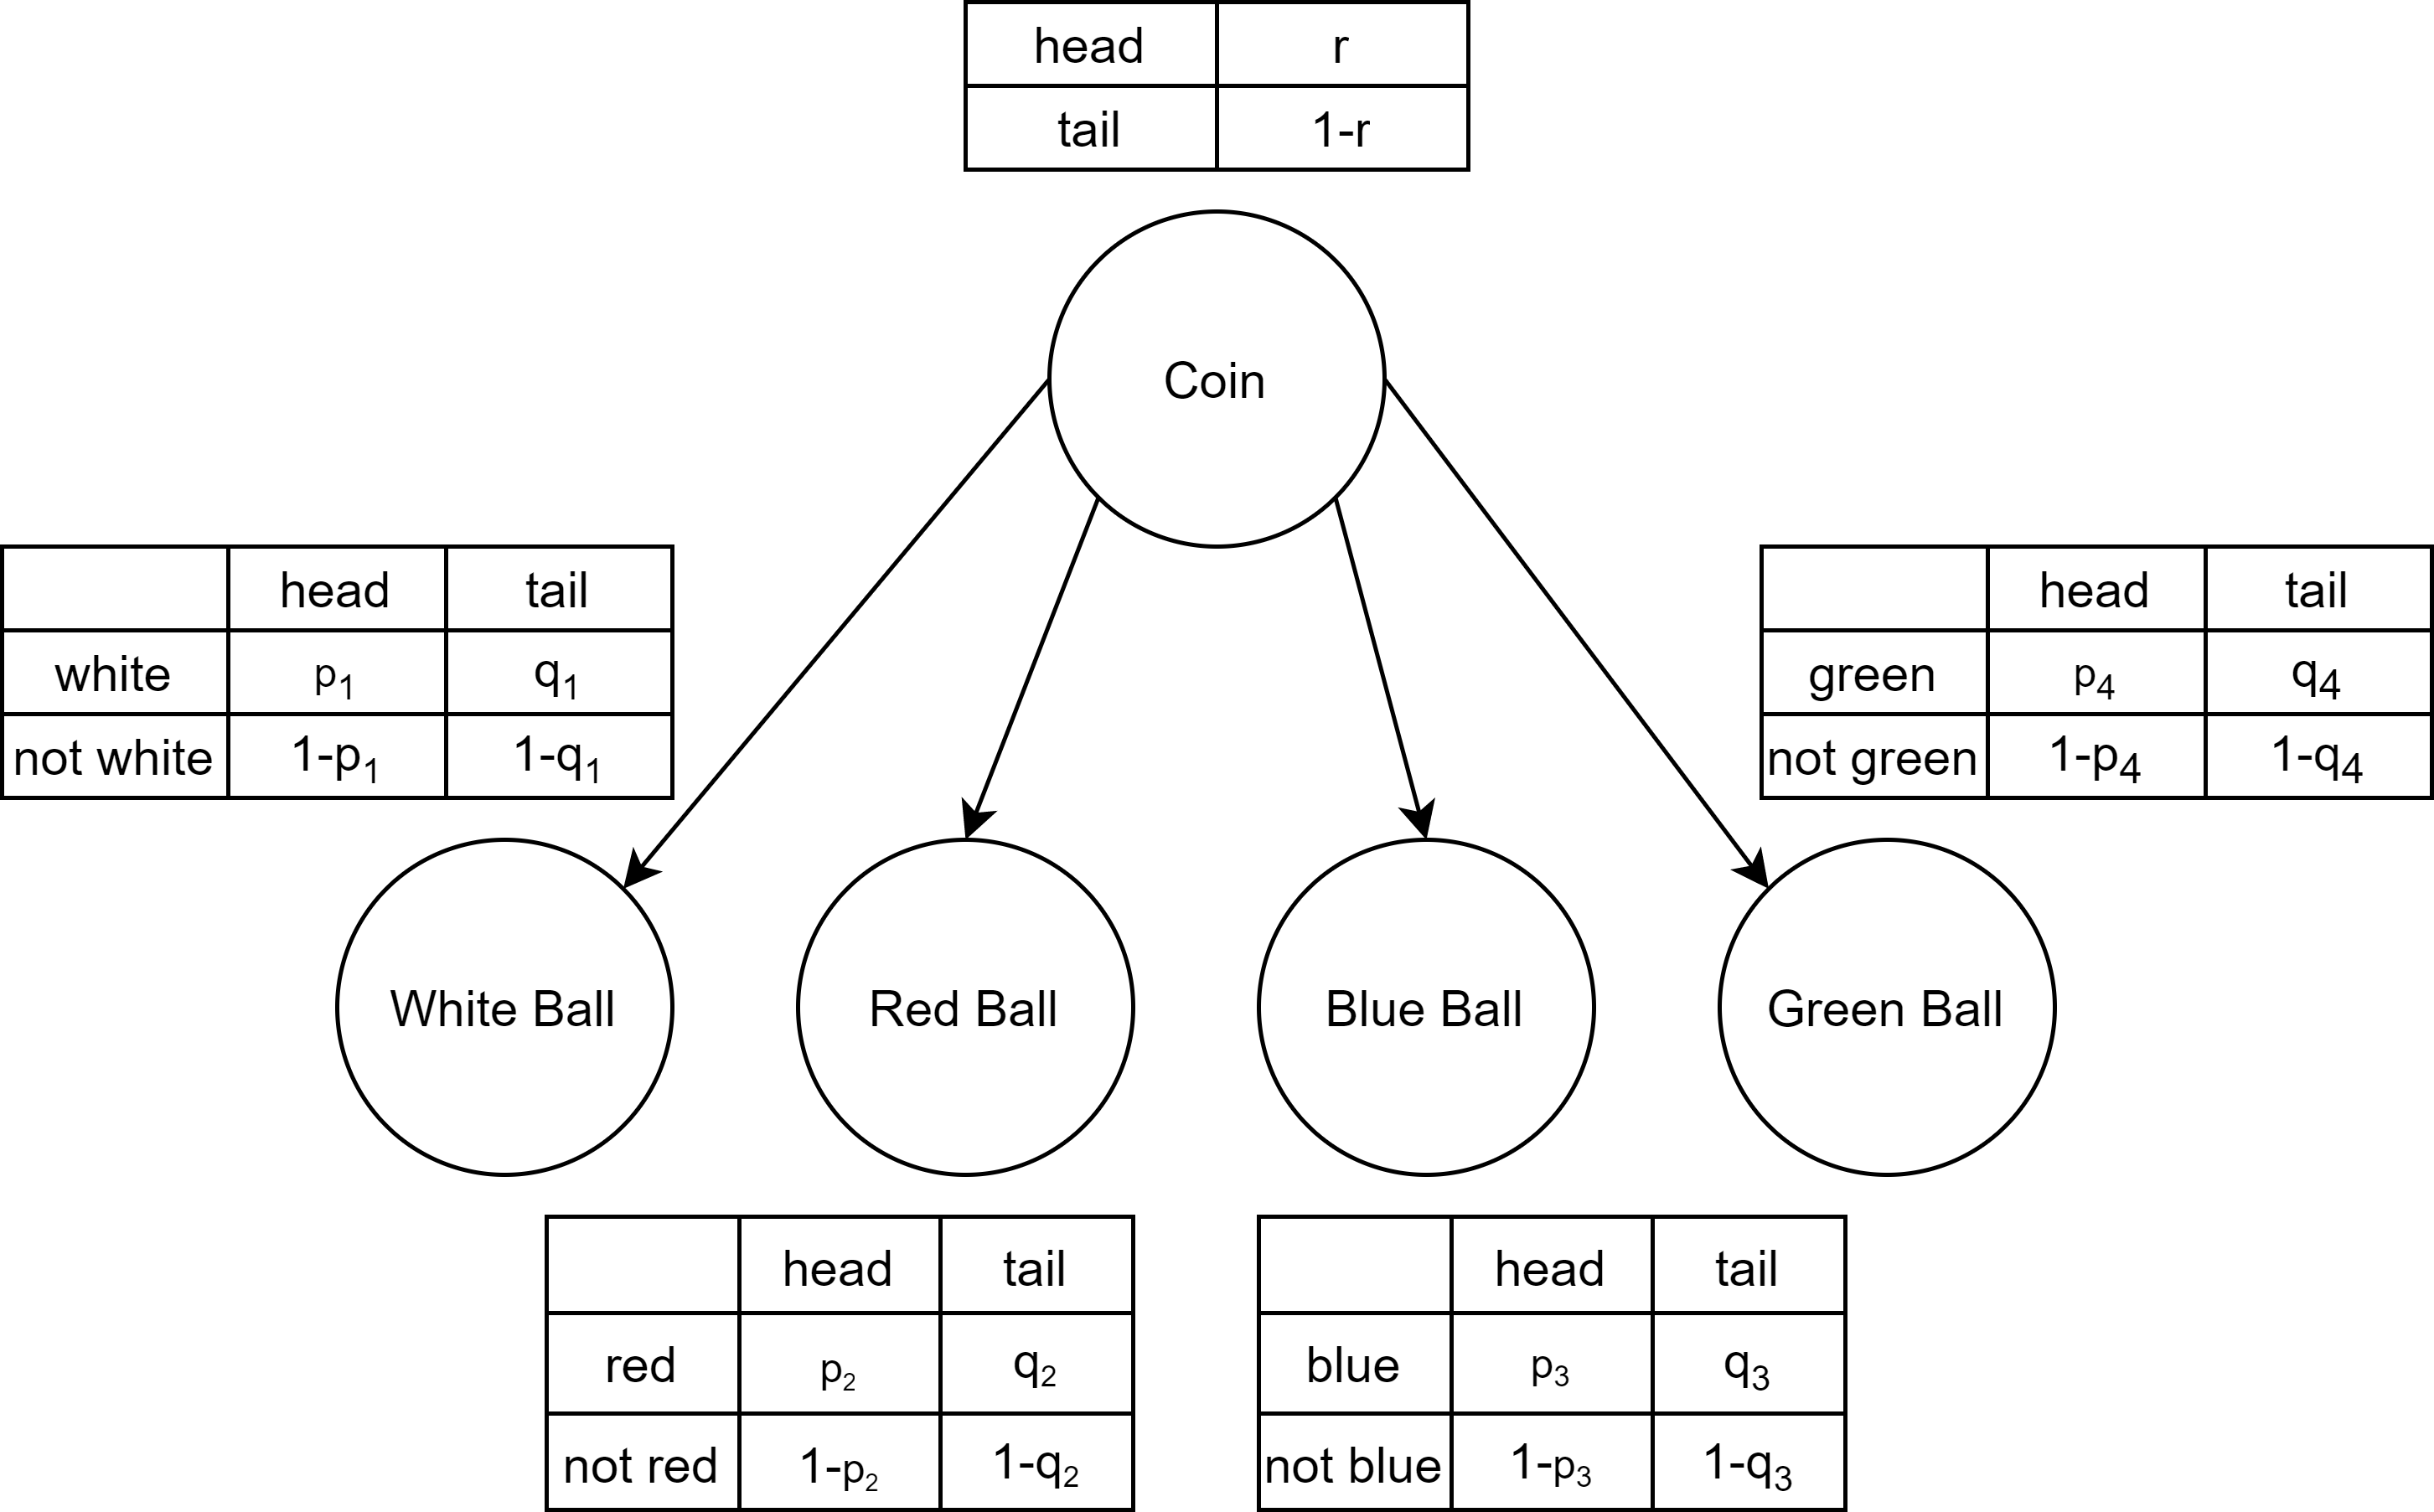
\includegraphics[width=\textwidth]{./assets/4-1.drawio.png}
    \caption{Bayes' network for each coin toss}
    \label{fig:bayes-net}
\end{figure}

\subsection{}
\begin{gather*}
    P(\text{Isochromatic}|\text{TTH}) = A \\
    \text{Isochromatic}: balls \in \{(w, w, w), (r, r, r), (b, b, b), (g, g, g)\} \\
    \text{TTH}: coins = \{T,T,H\} \\
    \Rightarrow A = \frac{P(\text{Isochromatic}, \text{TTH})}{P(\text{TTH})} \\
    = \frac{(1-r)^2 \times r \times (q_1 q_1 p_1 + q_2 q_2 p_2 + q_3 q_3 p_3 + q_4 q_4 p_4)}{(1-r)^2 \times r} \\
    = q_1 q_1 p_1 + q_2 q_2 p_2 + q_3 q_3 p_3 + q_4 q_4 p_4 \\
    = q_1^2 p_1 + q_2^2 p_2 + q_3^2 p_3 + q_4^2 p_4 \\
    = \sum_{i=1}^4 q_i^2 p_i 
\end{gather*}

\subsection{}
\begin{gather*}
    P(\text{H}|\text{Red}) = A \\
    \text{H}: coins = \{H\} \\
    \text{Red}: balls \in \{(r)\} \\
    \Rightarrow A = \frac{P(\text{H}, \text{Red})}{P(\text{Red})} \\
    = \frac{r p_2}{rp_2 + (1-r)q_2} 
\end{gather*}

\end{document}